\documentclass{article} \usepackage{amsmath} \usepackage{amssymb} \usepackage{amsthm} \usepackage[margin=0.2in]{geometry} \usepackage{hyperref} \usepackage{physics} \usepackage{tikz} \usetikzlibrary{decorations.pathmorphing} \usepackage{mathtools} \mathtoolsset{showonlyrefs} \theoremstyle{definition} \newtheorem{theorem}{Theorem}[section] \newtheorem{corollary}{Corollary}[theorem] \newtheorem{lemma}[theorem]{Lemma} \newtheorem{definition}{Definition}[section] \author{Connor Duncan} \date{\today}
\title{Physics-105-Lecture-Notes-04-23-2019}
\begin{document}
\maketitle\tableofcontents
\noindent\abstract{A single PDF with all lectures in a single document can be downloaded at \url{https://www.dropbox.com/sh/8sqzvxghvbjifco/AAC9LoSRnsRQDp7pYedgWpQMa?dl=0}. The password is 'analytic.mech.dsp'.
 This file was automatically generated using a script, so there might be some errors. If there are, you can contact me at \url{mailto:ctdunc@berkeley.edu}.}
\section{Nonlinear Mechanics + Chaos} You're gonna need to read the chapter and code to solve the majority of these problems. There are only a few of these that we can solve and understand analytically. \subsection{Van der Pol Oscillator} This is a van der pol oscilator. \begin{center} 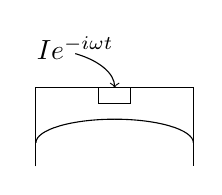
\begin{tikzpicture} \draw (-1,0)--(-1,1)--(1,1)--(1,0); \draw (1,0.3)arc(0:180:1 and 0.3); \draw (-0.2,1) rectangle (0.2,0.8); \draw[<-] (0,1) arc (0:60:1 and 0.5); \node (a) at (-0.5,1.5) {$Ie^{-i\omega t}$}; \end{tikzpicture} \end{center} \subsection{Duffing's Oscillator} \begin{center} 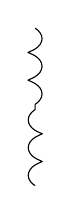
\begin{tikzpicture} \draw[decoration={coil},decorate] (0,1)--(0,0); \draw[decoration={coil},decorate] (0,-1)--(0,0); \end{tikzpicture} \end{center} two springs attached to a mass in a plane with relaxed length $l_0$. So we have \begin{align} U=\frac{1}{2}k(\sqrt{x^2+l^2}-l_0)^22 \end{align} which we expand to be (taylor about 0) \begin{align} \pdv{U}{x}=2k(\sqrt{l^2+x^2}-l_0)\left(\frac{1}{2}(l^2+x^2)^{1/2}2\lambda\right)=2k\left(x-\frac{xl_0}{\sqrt{l^2+x^2}}\right) \\ \pdv[2]{U}{x}=2k\left(1-\frac{l_0l^2}{(l^2+x^2)^{3/2}}\right) \\ \pdv[3]{U}{x}=6kl_0l^2(x^2+l^2)^{-5/2}x \\ \pdv[4]{U}{x}=\frac{6kl_0}{l^3} \end{align} So, when we put in the right taylor expansion coefficients, the effective potential beomes \begin{equation} U(x)\approx U(0)+k\left(1-\frac{l_0}{l}\right)x^2+\frac{1}{4}\frac{kl_0}{l^3}x^4+\ldots \end{equation} So the force becomes \begin{equation} F=-\pdv{U}{x}=-2k\left(1-\frac{l_0}{l^2}\right)x-\frac{kl_0}{l^3}x^3 \end{equation} There's a spring term, and a cubic term. So we want to solve the following differential equation \begin{equation} m\ddot x+2\beta m\dot x+2k\left(1-\frac{l_0}{l}\right)x+\frac{kl_0}{l^3}x^3=f(t) \end{equation} If we check this out in phase space, we look at \begin{center} 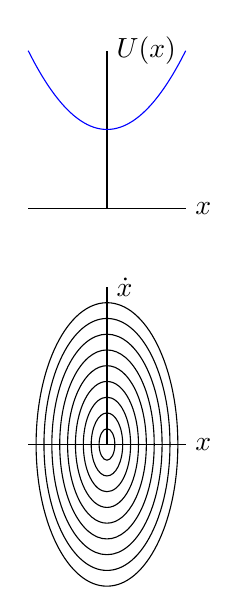
\begin{tikzpicture} \draw (-1,-1)--(1,-1) node[anchor=west]{$x$}; \draw (0,-1)--(0,1) node[anchor=west] {$U(x)$}; \draw[scale=1,domain=-1:1,smooth,variable=\x,blue] plot ({\x},{(\x)^2}); \draw (-1,-4)--(1,-4) node[anchor=west]{$x$}; \draw (0,-4)--(0,-2) node[anchor=west]{$\dot x$}; \foreach \r in {0,0.1,...,1} { \draw (0,-4) ellipse ({\r} and {\r/.5}); } \end{tikzpicture} \end{center} if we actially account for the cubic term in potential, however, we're going to get a taylor expansion that looks more like \begin{center} 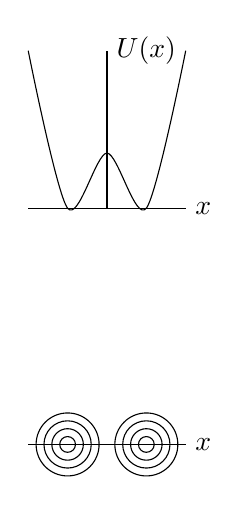
\begin{tikzpicture} \draw (-1,-1)--(1,-1) node[anchor=west]{$x$}; \draw (0,-1)--(0,1) node[anchor=west] {$U(x)$}; \draw plot [smooth] coordinates {(-1,1)(-.5,-1)(0,-.3)(.5,-1)(1,1)}; \draw (-1,-4)--(1,-4) node[anchor=west]{$x$}; \foreach \r in {0,.1,...,.5} { \draw (-.5,-4) ellipse (\r); \draw (.5,-4) ellipse (\r); } \end{tikzpicture} \end{center} i.e. there are multiple stable points in phase space. If we go back to solving this bad boi in generalit, we'll take \begin{equation} \ddot x+\frac{\dot x}{Q}+x+\epsilon x^3=f\cos\omega t \end{equation} Now, let's let $Q\rightarrow\infty$ so there's no damping, and fourier expand this, \begin{equation} x(t)=\sum_nA_n(\omega)\cos(n\omega t) \end{equation} with the differential equation being now \begin{equation} \ddot x+x+\epsilon x^3=f\cos(\omega t) \end{equation} So now, we want to take a look at the harmonics so we have (even terms go away since they correspond to the sin components)) \begin{align} x(t)=A_1\cos(\omega t)+A_3\cos(3\omega t)+\ldots \\ \dot x=-A_1\omega\cos\omega t-3\omega A_3\sin(3\omega t) \\ \ddot x=-\omega^2A_1\cos\omega t-9\omega^2A_3\cos\omega t \end{align} Making use of the trig id that \begin{equation} \cos^3x=\frac{3\cos(x)+\cos(3x)}{4} \end{equation} we have our differential equation as \begin{equation} \begin{matrix*}[r] (1-\omega^2)A_1\cos\omega t+(1-9\omega^2)A_3\cos(3\omega t)+\ldots \\ +\frac{\epsilon}{4}(3A_1^3\cos\omega t+A_1^3\cos(3\omega t)+\ldots) \\ =f\cos\omega(t) \end{matrix*} \end{equation} if we group our coefficients by $n$, we get \begin{align} (1-\omega^2)A_1+\epsilon\frac{3}{4}A_1^3=f\\ (1-9\omega^2)A_4+\epsilon\frac{1}{4}A_1^3=0 \end{align} So, graphically it looks a bit like \begin{center} \begin{tikzpicture}[scale=2] \draw (0,-1)--(0,1) node[anchor=west] {$A_1$}; \draw (-1,0)--(1,0) node[anchor=west] {$\omega$}; \draw (-1,0)--(1,1); \draw plot [smooth,tension=1] coordinates {(1,0.9)(0.2,0.4)(1,0.1)}; \end{tikzpicture} \end{center} where solutions are given as intersections of these curves. If we put damping back in, we have (i.e. $Q$ finite) \begin{align} x=a\cos\omega t+b\sin\omega t\\ \dot x=-a\omega\sin\omega t+\omega b\cos\omega t\\ \ddot x=-a\omega^2\cos\omega t-b\omega^2\sin\omega t=-\omega ^2x \end{align} , which gives us an equation from our initial requirements that \begin{equation} \begin{matrix*}[r] a(1-\omega^2)\cos\omega t+b(1-\omega^2)\sin\omega t+\frac{b\omega}{Q}\cos\omega t+\frac{3\epsilon ar^2}{4}\cos\omega t \\ +\frac{3\epsilon br^2}{4}\sin\omega t-\frac{a\omega}{Q}\sin\omega t\\ =f\cos\omega t \end{matrix*} \end{equation} which gives a solution for $r^2$ as a function of $\omega$ \begin{equation} r^2=\frac{f^2}{\left(1-\omega^2+\frac{3\epsilon r^2}{4}\right)^2+\frac{\omega^2}{Q^2}} \end{equation} which gives you pictures that kind of look like this \begin{center} 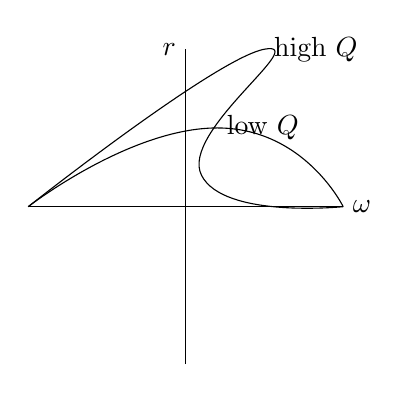
\begin{tikzpicture}[scale=2] \draw (0,-1)--(0,1) node[anchor=east] {$r$}; \draw (-1,0)--(1,0) node[anchor=west]{$\omega$}; \draw plot [smooth,tension=1] coordinates {(-1,0)(0.5,1)(.1,0.2)(1,0)}; \node[anchor=west] (h) at (0.5,1) {high $Q$}; \draw plot [smooth,tension=1] coordinates {(-1,0)(0.2,0.5)(1,0)}; \node[anchor=west] (l) at (0.2,0.5) {low $Q$}; \end{tikzpicture} \end{center} this gives rize to a field of study called catastrophe theory, in which there are discontinuous changes in phase and $r$. This is like magnetic fields and hystereisis. Look this up in free time.
\end{document}
